\documentclass[article,a4paper,oneside,10pt]{memoir}

% -------------------------------------------------------------------------- %
% Page Layout                                                                %
% -------------------------------------------------------------------------- %
\setlrmarginsandblock{0.142857111\paperwidth}{0.142857111\paperwidth}{*}
\setulmarginsandblock{0.111111111\paperheight}{*}{1.25}
\checkandfixthelayout
\newfixedcaption{\figcaption}{figure}
\newfixedcaption{\tabcaption}{table}
\captiontitlefont{\small}
\captionnamefont{\bfseries\small}
\captiondelim{: }

% -------------------------------------------------------------------------- %
% Bibliography                                                               %
% -------------------------------------------------------------------------- %
\renewcommand{\bibsection}{%
    \chapter{References}%
    \prebibhook}
\bibintoc
\renewcommand{\cftdot}{\textcolor{gray}{.}}
\renewcommand{\cftchapterdotsep}{\cftdotsep} % Chapters have dots in ToC
\renewcommand{\cftsectiondotsep}{\cftnodots} % Sections have no dots in ToC


% -------------------------------------------------------------------------- %
% Chapter and Section Headings                                               %
% -------------------------------------------------------------------------- %
\makeatletter
\makechapterstyle{alpensec}{%
  \chapterstyle{default}
  \setlength{\beforechapskip}{3.5ex \@plus 1ex \@minus .2ex}
  \renewcommand*{\chapterheadstart}{\vspace{\beforechapskip}}
  \setlength{\afterchapskip}{2.3ex \@plus .2ex}
  \renewcommand{\printchaptername}{}
  \renewcommand{\chapternamenum}{}
  \renewcommand{\chaptitlefont}{\sffamily\LARGE\bfseries}
  \renewcommand{\chapnumfont}{\chaptitlefont}
  \renewcommand{\printchapternum}{\chapnumfont \thechapter\quad}
  \renewcommand{\afterchapternum}{}}

\renewcommand{\section}{%
  \sechook%
  \@startsection{section}{1}%  level 1
      {\secindent}%            heading indent
      {\beforesecskip}%        skip before the heading
      {\aftersecskip}%         skip after the heading
      {\sffamily\secheadstyle}} % font

\makeatother

\chapterstyle{alpensec}


% -------------------------------------------------------------------------- %
% Packages                                                                   %
% -------------------------------------------------------------------------- %
\usepackage[%
        bookmarksnumbered=true,
        colorlinks=true,
        linkcolor=cyan!50!blue,
        citecolor=violet,
        urlcolor=purple,
    ]{hyperref}
\usepackage[light,nott]{kpfonts}
\usepackage{microtype}
\usepackage[english]{babel}
\usepackage[T1]{fontenc}
\usepackage[utf8]{inputenc}
\usepackage{xcolor-solarized}
\usepackage{lipsum}
\usepackage{graphicx}
\usepackage{minted}
\renewcommand{\listingscaption}{\small\bfseries Listing}


% -------------------------------------------------------------------------- %
% Macros                                                                     %
% -------------------------------------------------------------------------- %
\newcommand\code[1]{\texttt{#1}}


% -------------------------------------------------------------------------- %
% Title                                                                      %
% -------------------------------------------------------------------------- %
\title{\textsf{\Huge  The Black Magic of Floats in \LaTeX}}
\author{Raphael Frey\\[2mm]\small%
    \href{https://github.com/alpenwasser/TeX/tree/master/floats}
         {\nolinkurl{https://github.com/alpenwasser/TeX/}}}

\date{\vspace{1em}\today}

% ************************************************************************** %
\begin{document}
% ************************************************************************** %


\maketitle

\begin{abstract}
    The behavior  of floats can  often be  confusing for the  uninitiated, and
    yield  unexpected results. This  document gives  a brief  overview on  the
    subject, primarily based on Leslie  Lamport's \emph{\LaTeX{} -- A Document
    Preparation System} \cite{lamport}.

    I will not cover every possible edge case, but present some usage examples
    and common problem one tends to run into while working with floats.
\end{abstract}

\tableofcontents*
\listoflistings
\listoffigures
\listoftables


% ========================================================================== %
\newpage
\chapter{What Are Floats, Anyway?}
\label{chap:what-are-floats}
% ========================================================================== %

Normal text  is broken  by \TeX{} across  lines and  pages automatically. Some
content, such as images, are not  well-suited to being split into pieces. That
is what floating environments are for: To provide a way to put such content in
a place where it does not need to be broken; a way for it to \emph{float} to a
suitable location for an optimal overall result.

Two  such  floating environments  are  provided  by \LaTeX{}  by  default: The
\verb|figure|   and  the   \verb|table|\footnotemark  environment. There   are
packages   which  define   more  floating   environments  (for   example,  the
\verb|listings| packages can  let its code listings float, if  so desired), or
the user may define their own floating environments, if they so wish.

\footnotetext{%
    Because confusion is fun: The \texttt{table} environment does not actually
    typeset  a table.   That is  what \texttt{tabular},  \texttt{tabularx} and
    similar environments are for. See  \cite{mori:tables} for an overview. The
    \texttt{table}  environment is  merely a  floating container  intended for
    containing tabular content.}

Fundamentally, the only important difference between these environments is how
they  are  captioned  and  numbered: \verb|figure|  environments  will  get  a
different caption and  number to a \verb|table|  environment. However, one may
in principle put pretty much  anything one desires into either environment. As
long  as  the  code  itself  is  valid,  \LaTeX{}  will  not  complain. Figure
\ref{fig:lipsum} and Table \ref{lipsum} demonstrate this by placing some Lorem
Ipsum text inside their environments.

The floating behavior can be demonstrated by the fact that, in the source code
of this document, \ref{fig:lipsum} and \ref{tab:lipsum} are placed right after
this sentence. In the resulting document, they may be placed wherever \LaTeX{}
deems most suitable (maybe at the top of this page\footnotemark, maybe not).

\footnotetext{%
    \LaTeX{} usually tries  to place floats either  at the top of  a page, the
    bottom of a page, or on a separate page. See \ref{chap:placement} for more
    information.}


\begin{figure}
    \small\lipsum[2]
    \caption{A \texttt{figure} environment with placeholder text}
    \label{fig:lipsum}
\end{figure}

\begin{table}
    \caption{A \texttt{table} environment with placeholder text}
    \label{tab:lipsum}
    \small\lipsum[2]
\end{table}


Because  captions are  a moving  argument (Section  3.5.1 in  \cite{lamport}),
fragile  commands  such  as  linebreaks   inside  them  must  be  preceded  by
\verb|\protect|, as shown in the caption of Figure \ref{fig:protect}.

\begin{figure}
    \centering
    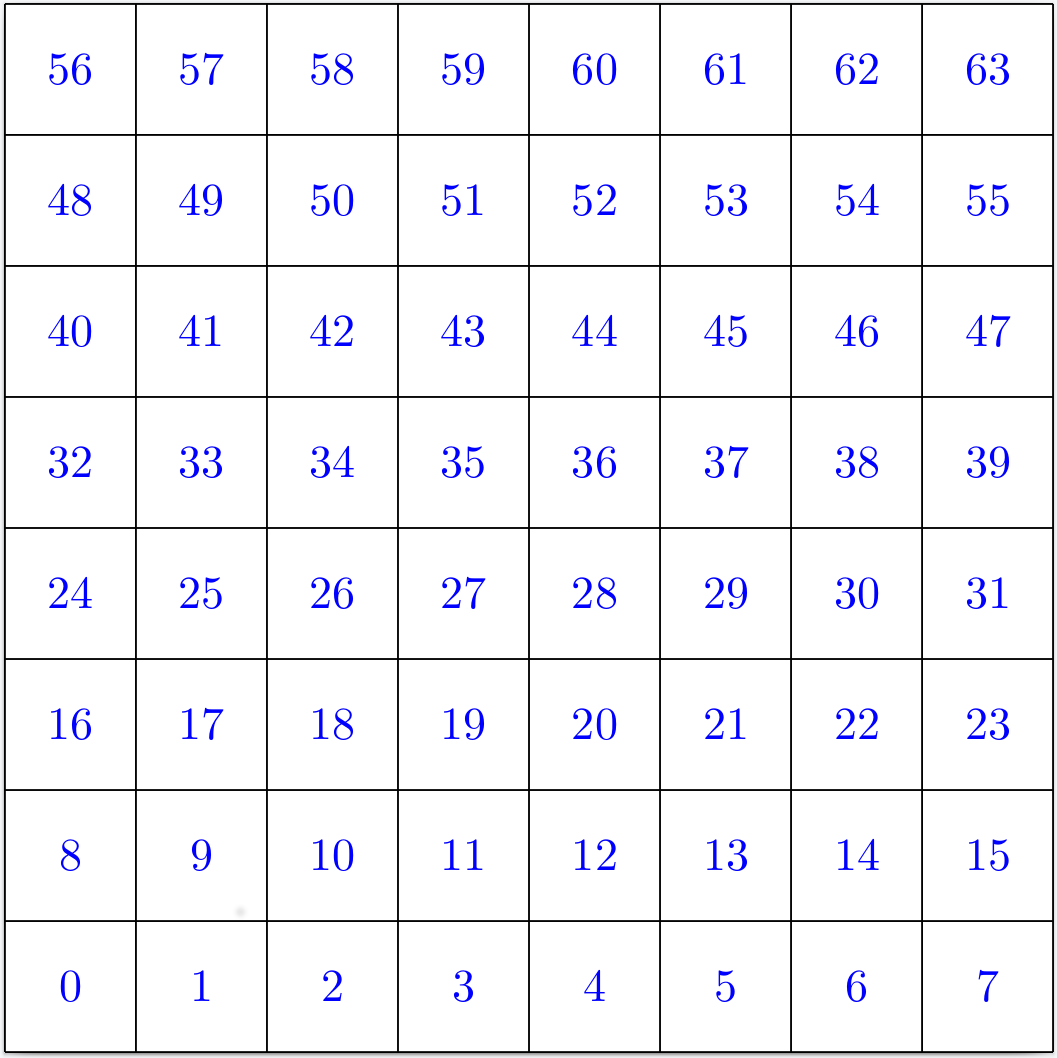
\includegraphics[height=3cm,width=4.5cm]{images/grid8cm.png}
    \caption[Linebreaks in Captions]{%
        One can  place arbitrary  content inside a  \code{figure} environment,
        though this does not usually make much sense.\protect\\
        Note      that       you      can      also       have      linebreaks
        inside     a      \code{caption},     but     it      requires     the
        \code{\textbackslash{}protect} command before  the linebreak, like so:
        \code{\textbackslash{}protect\textbackslash\textbackslash}}
    \label{fig:protect}
\end{figure}

The \verb|\caption| command can only be  used inside a floating environment by
default.   If  you require  captions  for  non-floating arguments,  there  are
packages which provide such facilities,  as well as more caption customisation
options,   see   \cite{ctan:package:caption,ctan:topic:caption}  and   Chapter
\ref{chap:alternatives} of this document.


% ========================================================================== %
\chapter{Basic Usage}
\label{chap:basic-usage}
% ========================================================================== %

Listing \ref{lst:figure}\footnotemark  shows the  basic code for  including an
external graphics file inside a \verb|figure| environment.

\footnotetext{%
    Incidentally, Listing \ref{lst:figure}  is one of those cases  where a new
    type  of floating  environment  has been  provided; in  this  case by  the
    \texttt{minted} package.}

\begin{listing}
    \begin{minted}[autogobble]{tex}
        \begin{figure}
            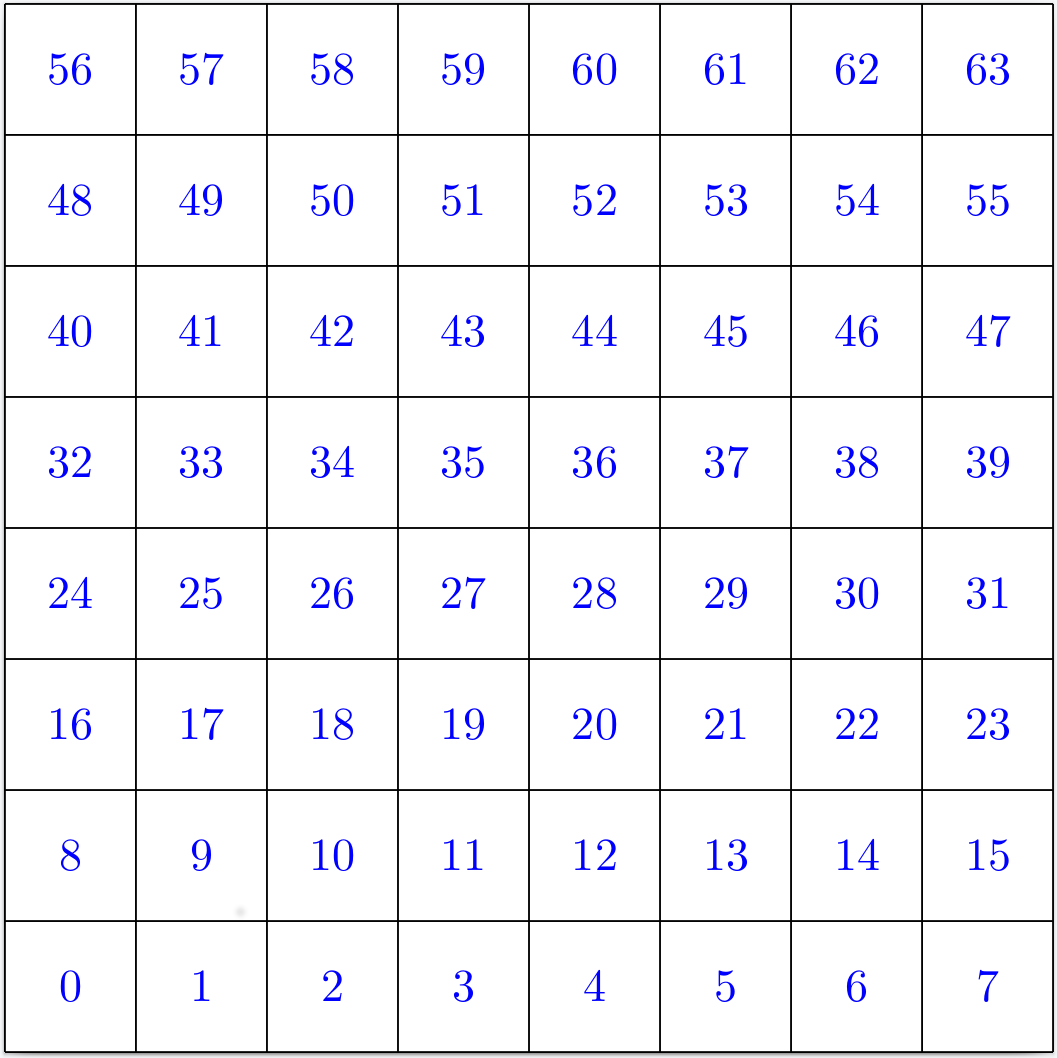
\includegraphics[height=3cm,width=4.5cm]{images/grid8cm.png}
            \caption{A very interesting and slightly distorted picture of a grid}
            \label{fig:distorted-grid}
        \end{figure}
    \end{minted}
    \caption{Code block for includeing a graphics in a figure}
    \label{lst:figure}
\end{listing}

It is  often desirable to center  a table or a  picture, in which case  we add
a  \verb|\centering|  directive  into  the environment,  as  done  in  Listing
\ref{lst:centering}\footnotemark.

\footnotetext{%
    There     exists     also    a     \texttt{\textbackslash{}begin\{center\}
    \ldots   \textbackslash{}end\{center\}}   environment. For  the   curious,
    some    information    on    the     differences    between    that    and
    \texttt{\textbackslash{}centering} can be found at
    \cite{stackexch:center-centering,texblog:center-centering}}


\begin{listing}
    \begin{minted}[autogobble,escapeinside=||]{text}
        \begin{table}
            |\textcolor{solarized-red}{\textbf{\textbackslash{}centering}}|
            \caption{Results for an experiment}
            \label{tab:experiment}
            \begin{tabular}{ll}
                \toprule
                Experiment Input  & Experiment Output        \\
                \midrule
                interesting thing & interesting result!      \\
                boring thing      & mildly surprising result \\
                weird thing       & very unexpected result   \\
                fascinating thing & machine broke            \\
                Xenomorph XX121   & dead scientists          \\
                \bottomrule
            \end{tabular}
        \end{table}
    \end{minted}
    \caption{%
        Centering  a  \texttt{tabular}   environment  inside  a \texttt{table}
        floating environment}
    \label{lst:centering}
\end{listing}

You may have noticed that the  \verb|\caption| is placed above the content for
tables  and below  the picture  in  a \verb|figure|  environment. This is  not
prescribed by  \LaTeX, obviously, and  will depend  on the style  guide you're
following or your own preferences. All I will  say on the subject is that most
tables I've seen  had their caption above  the table and most  images had them
below the picture.

\textcolor{solarized-red}{What   does   matter,    however,   is   where   the
\texttt{\textbackslash{}label}  is  put!} In  order  to pick  up  the  correct
number, it must  always come after the \verb|\caption| command  to which it is
supposed to  be connected. If you  put it before the  \verb|\caption| command,
the  \verb|\label| will  pick up  whichever counter  was the  last active  one
before the \verb|\caption|, which can be anything (another picture or table or
float of some sort, but also a chapter, section or similar). This is a mistake
which is easily made and often hard to detect.


% ========================================================================== %
\chapter{Placement Options}
\label{chap:placement}
% ========================================================================== %

So you have written  your document, or a large part of it,  and the floats are
just not  where you'd like  them to be? That  is where placement  options come
in. They allow you  to tell \LaTeX{} where  you would like your  floats to be,
with more  or less vehemence. It  will then try  to accomodate your  wishes as
best it can while still following its internal rules to some extent.

\textcolor{solarized-red}{Whatever  your   preferences,  only   use  placement
options  once your  text  is  (almost) complete.} Otherwise  you  will end  up
needing  to  change  them again  and  again  and  again,  causing a  lot  more
work. Also, it  is quite easily  possible to  overlook a bad  placement option
from  an earlier  version of  a document  which makes  you jump  through hoops
trying to get the best result even though \LaTeX{} would actually do the right
thing if you would just let it\footnotemark.

\footnotetext{%
    I am  obviously \emph{not}  speaking from  personal experience  here. I am
    smarter than that, I assure you.}


% ========================================================================== %
\chapter{Help, My Floats Are Jinxed!}
\label{chap:jinxed}
% ========================================================================== %

Too many floats, not enough text, \ldots


% ========================================================================== %
\chapter{\LaTeX's Dark Magic}
\label{chap:innards}
% ========================================================================== %


% ========================================================================== %
\chapter{Alternatives to Using Floats}
\label{chap:alternatives}
% ========================================================================== %


% ========================================================================== %
\newpage
\begin{thebibliography}{1}
% ========================================================================== %

    \bibitem{lamport}
        Leslie Lamport, Digital Equipment Corporation,
        ``\emph{\LaTeX{} -- A Document Preparation System}'',
        2nd Edition,
        1994,
        Addison-Wesley Publishing Company.

    \bibitem{mori:tables}
        Lapo Mori,
        ``\emph{Tables in \LaTeXe: Packages and Methods}'',
        The Prac\TeX{} Journal,
        2007-FEB-20.
        [Online],
        \href{https://www.tug.org/pracjourn/2007-1/mori/mori.pdf}
             {\nolinkurl{https://www.tug.org/pracjourn/2007-1/mori/mori.pdf}},
        [Accessed: 2017-MAR-27].

    \bibitem{ctan:package:caption}
        Comprehensive \TeX{} Archive Network.
        ``\emph{Package caption -- Customising captions in floating environments}''.
        [Online],
        \href{http://ctan.org/pkg/caption}{\nolinkurl{http://ctan.org/pkg/caption}},
        [Accessed: 2017-MAR-26].

    \bibitem{ctan:topic:caption}
        Comprehensive \TeX{} Archive Network.
        ``\emph{Topic caption}''.
        [Online],
        \href{http://ctan.org/topic/caption}{\nolinkurl{http://ctan.org/topic/caption}},
        [Accessed: 2017-MAR-26].

    \bibitem{stackexch:center-centering}
        Enrico Gregorio,
        ``\emph{When should we use \texttt{\textbackslash{}begin\{center\}} 
        instead of \texttt{\textbackslash{}centering?}}'',
        [Online],
        \href{http://tex.stackexchange.com/a/23653}
             {\nolinkurl{http://tex.stackexchange.com/a/23653}},
        [Accessed: 2017-MAR-26].
    
    \bibitem{texblog:center-centering}
        stefan,
        ``\emph{\TeX{}Blog -- center vs. centering}''.
        [Online],
        \href{http://texblog.net/latex-archive/floats/center-centering/}
             {\nolinkurl{http://texblog.net/latex-archive/floats/center-centering/}},
        [Accessed: 2017-MAR-27].

\end{thebibliography}

\end{document}
